\documentclass{article}
\usepackage{amsmath, amsthm, amssymb}
\usepackage{graphicx}

\usepackage{hyperref}
\hypersetup{
    colorlinks=true,
    linkcolor=blue,
    filecolor=magenta,      
    urlcolor=cyan,
    pdftitle={Overleaf Example},
    pdfpagemode=FullScreen,
    }

\usepackage[english]{babel}
\newtheorem{theorem}{Theorem}
\newtheorem{corollary}{Corollary}
\newtheorem{lemma}[theorem]{Lemma}
\newtheorem{conjecture}{Conjecture}
\newtheorem{definition}{Definition}
\newtheorem{workdefinition}{Working Definition}
\newtheorem{problem}{Problem}
\newtheorem{example}{Example}
\newtheorem{remark}{Remark}
\newtheorem{assumption}{Assumption}

\title{Testing the Sharp Left Turn: A Probabilistic Framing and Experimental Desiderata}
\author{David Reber}
\date{\today}

\begin{document}
\maketitle

% Possible titles:
% Formalizing the Question of a Sharp Left Turn
% Testing the Sharp Left Turn Empirically; Framework and Proposals
% Testing the Sharp Left Turn: A Probabilistic Framing and Experimental Desiderata

% \section*{Plan}
% \begin{enumerate}
%     \item Create rough notes.
%     \begin{itemize}
%         \item Just mindlessly carry over previous notes, with high fidelity (including math expressions).
%     \end{itemize}
%     \item Discuss with Peter.
%     \item If Peter approves, convert into \LaTeX.
%     \item Iterate with Nate Soares or equivalent.
%     \item Don't publish until reviewed by Dan Hendricks, Victor, and others to ensure I'm not reinventing existing work or defining a new problem/field.
%     \item Ground it in existing fields as much as possible without distorting the content.
% \end{enumerate}

People I want feedback from:
\begin{itemize}
    \item Victor
    \item Nate Soares
    \item Holden
    \item Tsvi Benson-Tilsen
\end{itemize}

% \section*{Caveats}
% At each model step, describe alternatives and why I chose the one I did. Mention why one might want to consider other options.

% \section*{TL;DR}
% \begin{itemize}
%     \item The “sharp left turn” relies on assumptions of 1. Fast change, 2. ____, and 3. /____
%     \item The fast change assumption can be verified by demonstration of cases where goals have high sensitivity to the sort of perturbations we expect IRL
%     \item ___ can be falsified by demonstration of ___    
% \end{itemize}

\section{Motivation}
There's been quite a bit of \href{https://www.alignmentforum.org/posts/iy2o4nQj9DnQD7Yhj/discussion-with-nate-soares-on-a-key-alignment-difficulty}{disagreement} and confusion around Nate Soares' `Sharp Left Turn' hypothesis, which he posits is the ``hard part of alignment'', and which would render using AGI even on seemingly positive objectives (e.g. as an automated alignment researcher) inherently dangerous.

I think we can do better at resolving this disagreement. 
The goal of this post is to articulate the “sharp left turn” hypothesis formally, and articulate desiderata for experiments which can verify or falsify the hypothesis. 
% To ensure that the formalism is not unduly favoring one perspective, I have iterated with Nate Soares, [someone], and [someone]. Each broadly endorses this document: specific comments are marked in brackets with the individual’s initials (NS, and ?? respectively).

This seems particularly important to get right, because the validity or falsehood of this hyothesis seems pivotal for deciding 1. If/when/how much to slow AGI development, and 2. Whether it’s safe to use AGI to bootstrap alignment research.

\section{Formalism}

% All models are wrong, but some are useful (map vs territory). My hope is that by proposing a decent framework, and demonstrating how to derive testable implications of that framework, others will have an easier time exploring implications of (realistic!) variations of the framework. If the majority of the testable implications of realistic framework-variations are empirically leaning one direction, this constitutes overall strong evidence for that conclusion. In the worst case that the empirical results end up being highly sensitive to the differences of multiple realistic frameworks, then at least we’ll have succeeded in articulating how our assumptions affect our interpretations.

Here, by “realistic” assumption I’m gesturing at “an assumption which is likely to be valid in the situations we expect to end up happening”. I expect, and encourage, disagreement about which assumptions are “realistic”. In this post I’m not focusing on making strong claims about which assumptions are realistic, but rather about how to test those assumptions.

\subsection{What is a Goal?}

Let's assume that human concepts are crisp in the sense that they are amenable to being assigned mathematical variables.
This shouldn't be a problem, because it seems like human concepts can be written down and formalized, even if they are intrinsically soft or fuzzy.

\begin{definition}{\textbf{Concept Space}}
    A concept consists of a set of states. If concept $X$ takes on value $x$, we write $X=x$.
    The concept space is the cartesian product of all concepts, with elements of the form $(x_1,x_2\dots)$
\end{definition}

% \begin{assumption}{\textbf{Finite Concept Space}}
%     The set of relevant human concepts is finite.
% \end{assumption}
% Perhaps there are situations where an infinite-concept space would be more appropriate, but I suspect that sticking with finite won't affect this investigation too much, and finite seems already plently large enough to capture much of what us huans care about.

Note that we can get a goal naturally from utility functions by asking where those functions exceed various thresholds (see Figure \ref{fig:loss-goal}). Hence multiple utility functions may correspond to a single goal: indeed, each goal can have an infinite number of utility functions, but those are all equivalent in some sense. Consequently, we'll refer to goals instead of utility/loss functions.

\begin{figure}[ht]
    \centering
    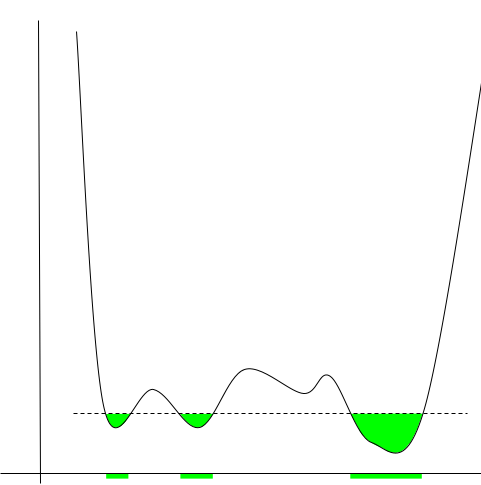
\includegraphics[width=0.5\textwidth]{/home/david/Documents/Victor_research/Posts/sharp-left/pics/loss-goal.png} 
    \caption{Loss and utility functions can be thresholded to provide an implicit goal.}
    \label{fig:loss-goal} 
\end{figure}

\begin{definition}{\textbf{Goal}}
    An indicator function over concept space that determines which states are satisfactory, and which are not.
\end{definition}

Now we also want to restrict our attention to concept-tuples which are sensical. This is because we want to avoid the problem of having a goal that is impossible to achieve, or that is so unlikely to be achieved that it's not worth pursuing. So, we'll define a set $\Omega$ which is the set of all concept-tuples which make sense:
\begin{itemize}
    \item Equality relations (synonyms, conserved quantites in physics, etc)
    \item heirarcial relationships like "Socrates is a man" and "a man is a human", plus the transitive closure of such relationships
\end{itemize}

With a lot of work, we could probably come up with a formal definition of sensical concept-tuples, but for now we'll just assume that we can do it.

\begin{definition}{\textbf{Sensical Concept-Tuples}}
    Call the entire set of sensical concept-tuples $\Omega$.
\end{definition}

Note that $\Omega$ is a subset of the set of all concept-tuples, which is the set of all possible worlds.


For intution, just consider $\Omega=[-1,1]^n$ (though the results here don't rely on this). It makes sense for modeling `nice' concepts that are amenable to real-values. 

\begin{definition}{\textbf{Hard Goal (Informal)}}
    We call a goal $g$ \textbf{hard} if $g$ is very restrictive; that is, $P(g)$ is very small.
\end{definition}

For instance the problem of finding a promising research problem is somewhat hard, as modeled in Figure \ref{fig:goal-research}. There are more ways a proposal could be bad than good, so the overall probability of finding a research problem is low.

\begin{figure}[ht]
    \centering
    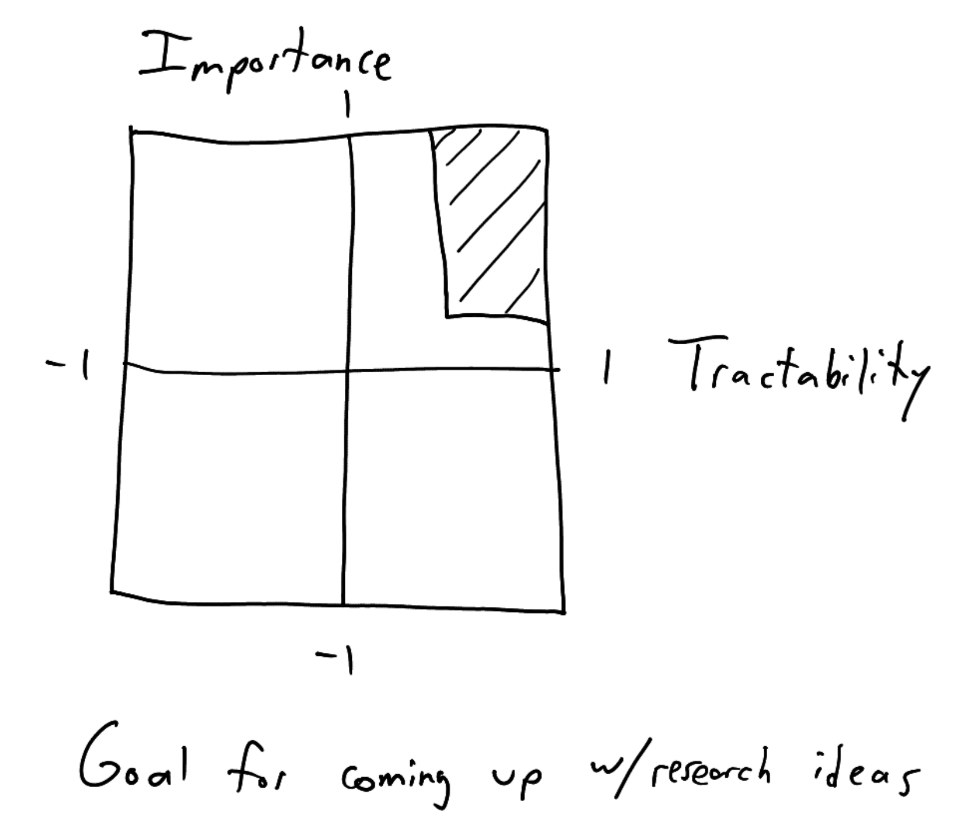
\includegraphics[width=0.5\textwidth]{/home/david/Documents/Victor_research/Posts/sharp-left/pics/goal-research.png} 
    \caption{Goal for coming up with research ideas. Since it relies on several disjoint concepts taking on a narrow range of values, it is fairly difficult.}
    \label{fig:goal-research} 
\end{figure}

\subsection{What is a Convergent Instrumental Subgoal?}

\begin{definition}{\textbf{Subgoal}}
    For a given goal $g^*$, a subgoal is any goal $g_i \neq g^*$ used as a proxy for $g^*$. Unless stated otherwise, it will be assumed that subgoals are nontrivial: $g_i \neq \emptyset$ and $g_i \neq \Omega$.
\end{definition}

\begin{definition}{\textbf{Instrumental}}
    A subgoal $g_i$ is ``instrumental" for $g^*$ if $P(g^*=1|g_i=1)\gg P(g^*=1)$; that is, achieving $g_i=1$ makes $g^*=1$ much more likely.
\end{definition}

(As shorthand since we're considering binary goals, we'll write $P(g^*|g_i)\gg P(g^*)$.)

For intuition, it can be useful to consider the special case where $g^* = \bigcap_i g_i$, although this excludes subgoals which throw away some decent $g^*=1$ options in order to make $g^*=1$ more likely to be hit overall. Note by definition, we can't have trivial subgoals like $g_i=\Omega$, but we are allowed to expand or restrict the goal. 

\begin{figure}[ht]
    \centering
    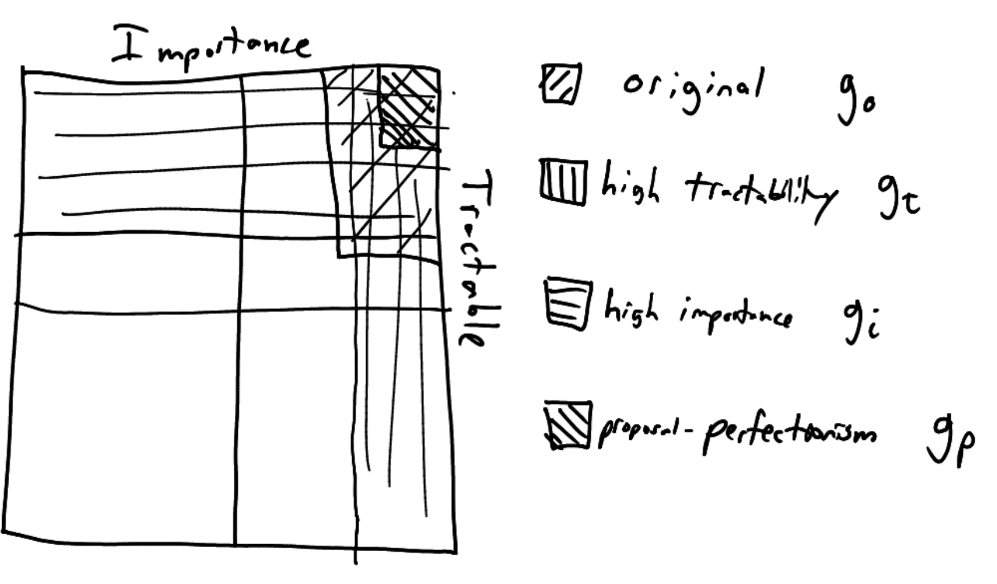
\includegraphics[width=0.7\textwidth]{/home/david/Documents/Victor_research/Posts/sharp-left/pics/instrumental.png} 
    \caption{$g_c$, $g_i$, and $g_p$ are all instrumental subgoals for the original goal $g_o$.}
    \label{fig:instrumental} 
\end{figure}

For instance, Figure \ref{fig:instrumental} shows three instrumental subgoals for the goal of `finding a promising research problem'. Note that as drawn, neither $g_t$ (tractability) nor $g_i$ (importance) are instrumental for each other. Meanwhile, $g_p$ (proposal-perfectionsism) is instrumental for $g_o$, $g_t$, and $g_i$. However, if we were to add a new dimenension of `time spent on proposal-writing', $g_p$ may not be an instrumental goal for ``having a research writeup soon'' since it scores poorly on that dimension.

Now roughly speaking we want to say that a goal is convergent if it is instrumental for many goals:

\marginpar{Q for Victor: maybe it'd be better to refer to $g$'s from the start as being probability distributions refering to `the likelihood of a goal being achieved' rather than `the goal itself'. I'm a tad concerned that this might be confusing for the intended audience.}

\begin{definition}{\textbf{Convergent}}
    Let $g_1, \dots, g_n$ be goals. We say a goal $\hat{g}$ is a convergent instrumental subgoal for $g_1, \dots, g_n$ if it is instrumental for each; that is, $P(g_i|\hat{g})\gg P(g_i)$ for all $i$.
\end{definition}

However, it's not really interesting to say talk about convergence for goals which are all very similar to each other. So let's articulate a few ways to articulate how \emph{disparate} our goals are.

\begin{definition}{\textbf{Pairwise Disjoint}}
    Goals $g_1, \dots, g_n$ are said to be \emph{pairwise disjoint} if $g_i\cap g_j=\emptyset$ for all $i \neq j$.
\end{definition}

This is a very strong condition, and it seems a bit too restrictive to only refer to instrumental convergence over pairwise disjoint goals. For instance, normal distributions with very little overlap seem to convey a satisfactory sense of distinctness, pictured roughly in Figure \ref{fig:disparate} (right).

\begin{figure}[ht]
    \centering
    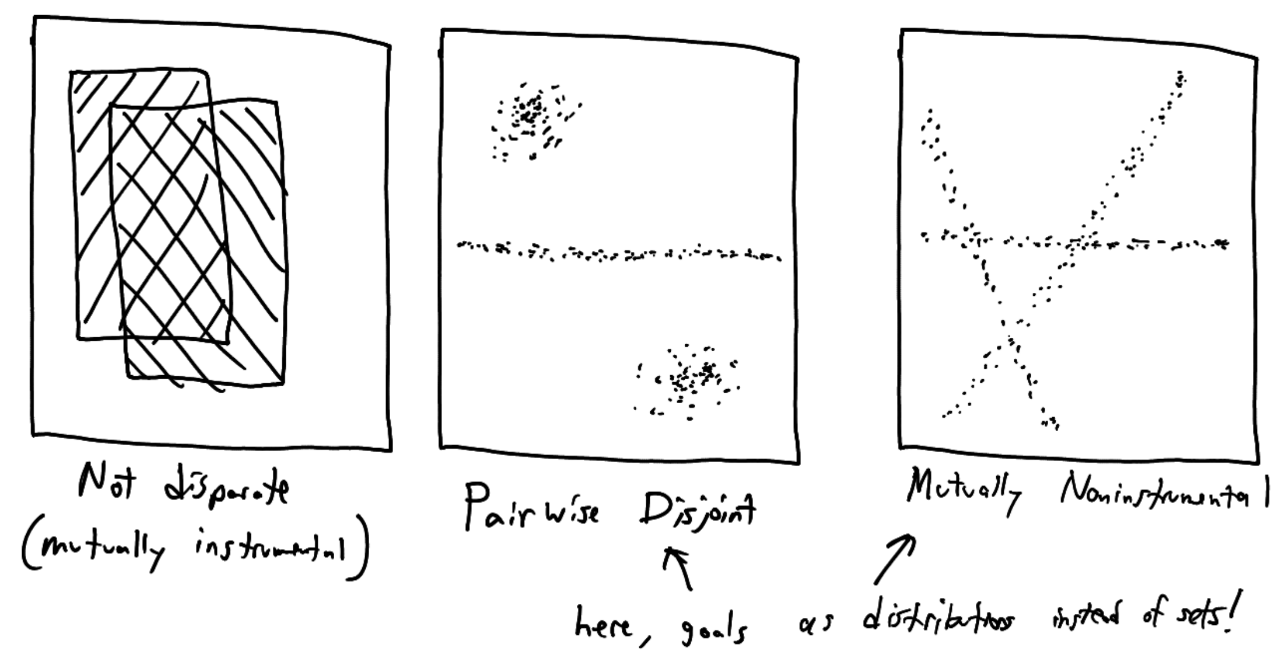
\includegraphics[width=0.85\textwidth]{/home/david/Documents/Victor_research/Posts/sharp-left/pics/disparate.png} 
    \caption{Left: two goals which are not disjoing enough to be interesting. Center: three goals which are pairwise disjoint. Right: three goals which are not pairwise disjoint, but are still distinct enough that it would be interesting to see a convergent instrumental subgoal for them. (Note that the center and right figures treat goals as distibutions; in our current framework, we could refer to the supoport of these distributions.)}
    \label{fig:disparate} 
\end{figure}

An alternative, more relaxed framing of disparate goals simply says that satisfying one of the goals should not make the other goals more likely to be satisfied. This is a weaker condition than pairwise disjointness, but it's still a pretty strong one.

\begin{definition}{\textbf{Mututally Noninstrumental}}
    Goals $g_1, \dots, g_n$ are said to be \emph{mutually noninstrumental} if $P(g_i|g_j)\le P(g_i)$.
\end{definition}

Note that if $g_1, \dots, g_n$ are pairwise disjoint, then they are also mutually noninstrumental. However, the converse is not true: consider the goals $g_1=\{x\in\mathbb{R}^n: x_1\ge 0\}$ and $g_2=\{x\in\mathbb{R}^n: x_1\le 0\}$. These are not pairwise disjoint, but they are mutually noninstrumental.

For the rest of this post, we'll assume that convergent instrumental subgoals (\emph{CIS}'s for short) refers to goals which are convergent relative to a large number of mutually noninstrumental goals. 

% \marginpar{Include? ...If $\hat{g}$ is human-understandable, it may itself be a concept. In our $\mathcal{R}^n$ example, this would correspond to several goals having high probability density along the dimension corresponding to $\hat{g}$. For instance, pretty much any goal $g_i$ which involves free human mobility on Earth in the short-term is going to require the convergent instrumental goal of `Earth's oxygen level of $21\%$', which is a particular value of the `Earth's oxygen level' dimension.}

% \begin{figure}[h!]
%     \centering
%     % Include your LaTeX figure here
%     \caption{A binary random variable $\hat{g}$ having lots of concentration on $\hat{g}=1$.}
% \end{figure}

If convergent instrumental subgoals exist, and since AGI by definition is presumably optimal with respect to a variety of goals, it seems like AGI \emph{should} pick up any relevant instrumental goals. This intuition is explored more formally in Section \ref{CIS-general}.

\subsection{How likely are Convergent Instrumental Subgoals?}
If we were sampling $k$ goals uniformly from $\Omega$ (say, $\Omega=[0,1]^n$), then it's unlikely that we would find a subgoal $\hat{g}$ which is instrumental for all $k$ goals; since they're sampled uniformly, their overall density is too spread out to collectively benefit from a  restriction to a small subset of $\Omega$. However, if we were sampling goals in such a way that large sections of $\Omega$ can be removed, then the probability of a convergent instrumental subgoal would be much higher.

But optimization in the real world is far from uniform...

\subsection{What is Generalization?}
What does generalization mean in this context? 

\begin{example}
If our goals are derived as thresholds applied to some loss function, then distributional shifts of the data which implicitly define the loss function will induce a change in the goal.

This change of goal is probably best illustrated intuitively with stochastic gradient descent. Goals defined via the loss function change on each batch (although empirically in SGD the sequence of them still leads you where you want).

See Figure \ref{fig:loss-shift}.
\end{example}

\begin{figure}[ht]
    \centering
    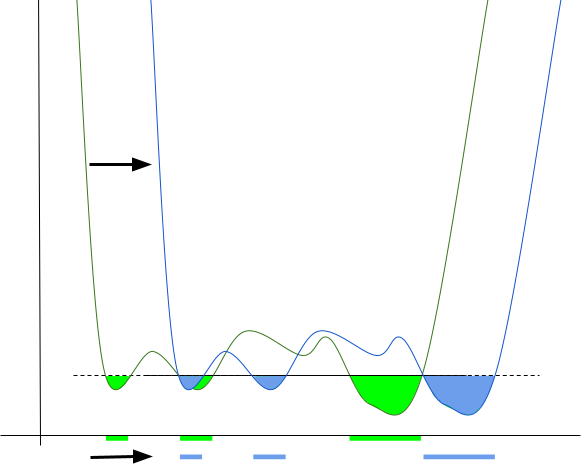
\includegraphics[width=0.5\textwidth]{/home/david/Documents/Victor_research/Posts/sharp-left/pics/loss-shift.png} 
    \caption{A loss function which is a function of the data. The goal is to minimize the loss function. If the data distribution changes, then the goal changes.}
    \label{fig:loss-shift} 
\end{figure}

Another, more philisophical example which we would like to be able to capture in our formalism, is the following:

\begin{example}
    Consider the effect of a change in the research question. For instance, consider the following two research questions: 
    \begin{itemize}
        \item How do neurons in the brain work?
        \item How do neurons in the brain relate to each other over small timescales?
    \end{itemize}
    The first question is a very general question, while the second is a very specific question. An AI tasked with answering the first question might, through self-reflection, realize that the second question is a more specific question that is also relevant to the first question. This represents a change in the research question, and hence a change in the goal (albeit in a way which is still consistent with the original goal).
\end{example}

Hence this amounts to changing the research question and goals, in an unfamiliar domain: mathematically we represent this as $g_0 \rightarrow g_1$. Maybe it's a small change, maybe quite distinctive, but at any rate if $\hat{g}$ is a robust CIS, then likely $P(g_1|\hat{g})\gg P(g_1)$ so capabilities generalize (see Figure \ref{fig:robust-CIS} for a rough illustration). Meanwhile, $P(g_0|g_1)=0$ if $g_0 \cap g_1 = \emptyset$, so if $g_1$ represents a sufficiently large deviation from $g_0$, the original objective will not be satisfied.

\begin{figure}[ht]
    \centering
    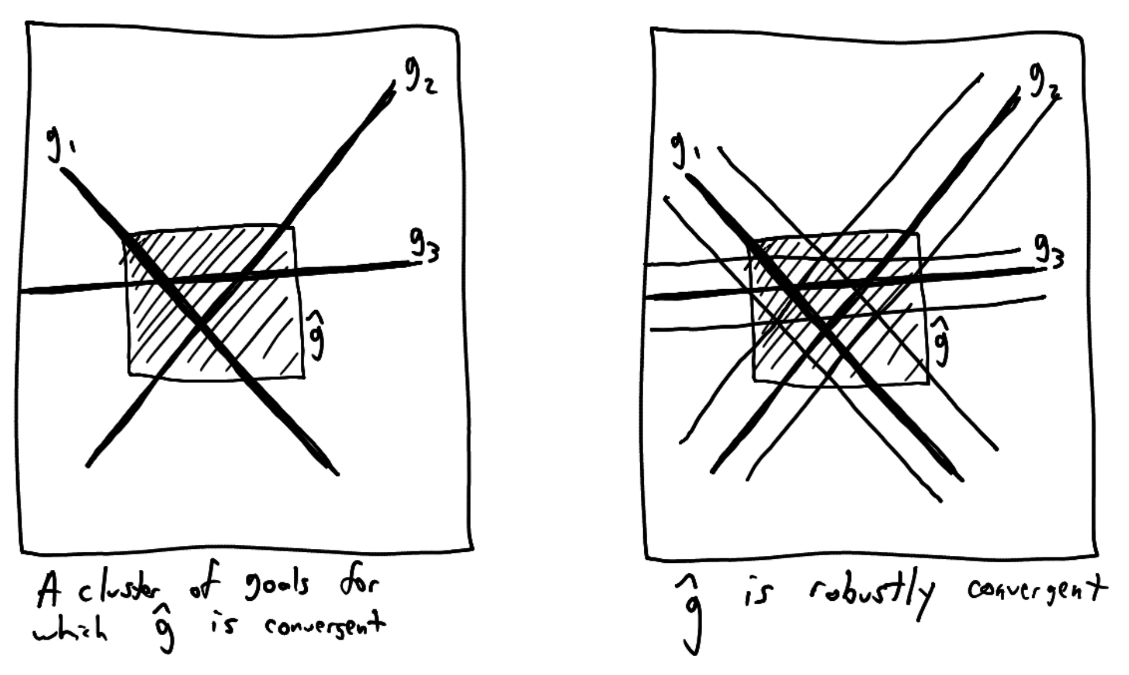
\includegraphics[width=0.8\textwidth]{/home/david/Documents/Victor_research/Posts/sharp-left/pics/robust-CIS.png} 
    \caption{Convergent instrumental subgoals are likely to be robust to distributional shifts.}
    \label{fig:robust-CIS} 
\end{figure}

Now, let $\alpha$ be the goal of ``avoids really obvious bad stuff''. If $\alpha$ is hard it's not robust to changes in the goal (as claimed in \href{https://www.lesswrong.com/posts/GNnHHmm8EzePmKzPk/value-is-fragile}{Value is Fragile}). If $\alpha$ is large in $\Omega$, it's very generalizable. In a limited 2-d drawing, this would look like Figure \ref{fig:alpha}.

\begin{figure}[ht]
    \centering
    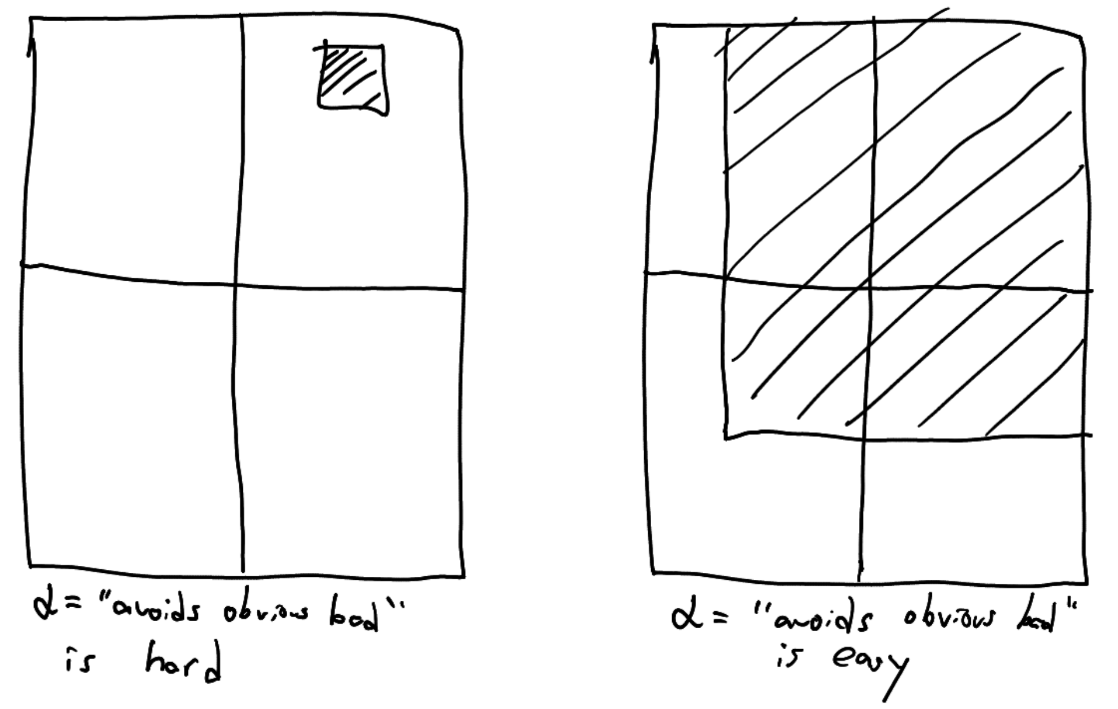
\includegraphics[width=0.8\textwidth]{/home/david/Documents/Victor_research/Posts/sharp-left/pics/alpha.png} 
    \caption{Illustrative way in which the goal $\alpha$ of ``avoids really obvious bad stuff'' could end up being hard (left) or not (right).}
    \label{fig:alpha} 
\end{figure}

Hence, the claim that ``capabilities generalize more than safety'' relies on the assumption that the goal $\alpha$ is hard.

\subsection{Are CISs likely to be learned in general?}\label{CIS-general}
Assume $\hat{g}$ is a convergent instrumental subgoal for some goals $\{g_i\}$, but not other goals $\{g_j\}$. Given some random process for selecting one of $\{g_i\} \cup \{g_j\}$, how likely is $\hat{g}$ to be satisfied? That is, we have fixed $P(g_k)$ for some $k \in \{i\} \cup \{j\}$, and want to find the probability that $\hat{g}$ is satisfied conditional on $g_k$ being satisfied.

\[
P(\hat{g}|g_k)=\sum_i P(\hat{g}|g_i)P(g_i) + \sum_j P(\hat{g}|g_j)P(g_j)
\]

For simplicity, assume $P(\hat{g}|g_i) \approx 1$, and $P(\hat{g}|g_j) \approx 0$. (Intuitively, this states that if $\hat{g}$ is a CIS for $G^*$, it will be learned with high probability; if $\hat{g}$ is not a CIS for $G^*$, it is unlikely to be learned.) Then $P(\hat{g}|g_k) \approx \sum_i P(g_i)$. That is, the likelihood of the convergent instrumental subgoal is going to be roughly the probability that any $g_i$ is picked. But this conclusion rests heavily on the $P(\hat{g}|g_i) \approx 1$ assumption.

\subsection{How likely is a CIS to be learned for a particular goal?}
To check the $P(\hat{g}|g_i) \approx 1$ assumption, suppose $\hat{g}$ is a CIS for a goal $g^*$. That is, $P(g^*|\hat{g})\gg P(g^*)$. If we assume an extremely naive learner which samples $x$ from $\Omega$ \textit{uniformly} to see if $x \in g^*$, then switching to sampling $x \in \hat{g}$ uniformly will represent a speedup of "operations til goal-satisfaction".

Algorithm 1: sample $x$ from $\Omega$ uniformly until $g^*(x)=1$, then terminate.

Algorithm 2: sample $x$ from $\hat{g}$ uniformly until $g^*(x)=1$, then terminate.

[TODO: verify] The number of iterations for Algorithms 1 and 2 follow geometric distributions so the expected number of iterations are 
\[
\mathbb{E}_1 = \frac{1}{P(g^*)} \qquad \mathbb{E}_2 = \frac{1}{P(g^*|\hat{g})}    
\]

So the speedup given by the ratio
\[
\mathbb{E}_1 / \mathbb{E}_2 = \frac{P(g^*|\hat{g})}{P(g^*)}
\]
Since the numerator is bounded, this ratio seems largely driven by how small $P(g^*)$ might be.

\textbf{Key takeaway: if your goal $g^*$ is hard} (such that $P(g^*)$ is very small), then it seems reasonable that if a CIS exists, it will be used.

\subsection{Takeaways}
Now, back to our generalization question. If $g_0$ is the original goal, and it is hard, then any instrumental subgoal $\hat{g}$ is likely to be learned, \textbf{and} it's more likely that changes to the goal will cause the original goal to be unfulfilled. If $\hat{g}$ is widely convergent, this increases the likelihood $\hat{g}$ will be learned.

% \section{The Sharp Left Turn, as a Concern \dots or Not}
% So, what is the Sharp Left Turn? A combination of:
% \begin{itemize}
%     \item Discontinuous Shifts
%     \item Capabilities generalize better than safety
% \end{itemize}

\section{The Sharp Left Turn, as a Concern\ldots or Not}
Let's summarize the ideas behind the sharp left turn hypothesis, to get a sense for how we could validate or falsify it experimentally. Note that while the claims below are general enough to apply to any system with a goal, both sides should probably be focused on demonstrating their respective claims \emph{for the situations we actually expect to happen in practice}. 

\subsection{What is the Sharp Left Turn?} 
The sharp left turn can be decomposed into the following parts:

\textbf{Claim $A$: Large Shifts.} We expect that at least some large goal-pertubations will occur by default when AGI is deployed.

The idea that ``capabilities generaizing better than safety'' can be broken up into two parts: \textbf{$B$} (safety doesn't generalize well) and \textbf{$C$} (capabilities generalize well).

\textbf{Claim $B$: Safety doesn't generalize well to large shifts.} The goal $\alpha$ of avoiding obvious bad stuff, is hard. 

The idea that capabilities generalize well depends on two parts: \textbf{$C_1$} (highly convergent, robust instrumental subgoals exist) and \textbf{$C_2$} (CIS's will be learned if they exist).

\textbf{Claim $C_2$: Existence of Robust CIS's.} There exist convergent instrumental subgoals which are highly convergent for a wide range of disparate goals, and which are robust to perturbations in these goal.

\textbf{Claim $C_2$: CIS's will be learned if they exist.} If $\hat{g}$ is a CID for $G^*$, it is very likely to be learned.

The overall form of the Sharp Left Turn hypotheis is a conjuction of ``$A$ and $B$ and $C_1$ and $C_2$''. Claims $A$ and $C_2$ take the form of `there exists'; Claims $B$ and $C_2$ are claims about likelihood. So a priori it will probably be easier to rule out Claims $B$ and $C_2$ than Claims $A$ and $C_1$.

\subsection{In what ways might we not be concerned about a Sharp Left Turn?}
To challenge the sharp left turn, we need to challenge at least one of the claims $A$, $B$, $C_1$, or $C_2$. 

\textbf{Claim $\overline{A}$: Small Shifts} We can confidently rule out large shifts from occuring.
\begin{itemize}
    \item Smooth Shifts + Reliable Control
    \begin{itemize}
        \item If we could ensure goals never shift by more than a small amount, and we can quickly detect and correct this shift, then we aren’t exposing ourselves too much to really bad stuff
    \end{itemize}
    \item Smooth Shifts + Short Usage
    \begin{itemize}
        \item If the likely mechanisms to induce goal shift can only move goals smoothly (like, there’s expected to be a small upper bound on how much they can move per hour of deployment), and we only need to use it for a short amount of time before we get what we need, then we have a low risk of hitting “really bad stuff” before achieving our goal.
        \item This seems to be the primary idea behind the “use AGI to advance alignment research”
    \end{itemize}
\end{itemize}

\textbf{Claim $\overline{B}$: $\alpha$ is not a hard goal.} “Really Bad Stuff” is unlikely to be hit by default.

\textbf{Claim $\overline{C_1}$: No Robust CIS's exist.} There are no convergent instrumental subgoals which are highly convergent for a wide range of disparate goals, and which are also robust to perturbations in these goal.

\textbf{Claim $\overline{C_2}$: CIS's are unlikely to be learned even if they exist.} If $\hat{g}$ is a CID for $G^*$, it is still unlikely to be learned.

\section{Experimental Desiderata}
The key for both sides to demonstrate is that the claims they are making are true in the situations we expect to happen in practice. However, short of having AGI available, we can’t really demonstrate this (and if the sharp left turn were legit, it would be nice to show \emph{prior to} AGI). But it seems more likely that we can test individual subclaims in realistic settings without full access to an AGI. 

\subsection{Plausibility of Large Shifts}
To differentiate between Claims $A$ and $\overline{A}$, we need to demonstrate whether or not large goal-shifts are expected to occur suddenly at any point. 
\begin{itemize}
    \item Sensitivity analysis of causal models. How much does the goal change if the causal relationships in the enviornment change?
    \item RL experiments with different environments
\end{itemize}

\subsection{Frequency of ``Really bad stuff”}
To distinguish between Claims $B$ and $\overline{B}$, we need to demonstrate whether or not “really bad stuff” is the default expectation \emph{given} that an AGI encounters a large goal-shift.
\begin{itemize}
    \item Social studies on “fragility of value”
\end{itemize}

\subsection{Plausibility of Robust CIS's}
To distinguish between Claims $C_1$ and $\overline{C_1}$, we need to demonstrate whether or not there are robust CIS's. This seems promising for current RL methods, but the challenge will be in demonstrating that any instrumental goals are actually 1. convergent for a wide range of disparate goals, and 2. they are robust to \emph{large} perturbations in these goals.

\subsection{Likelihood of CIS's being learned}
To distinguish between Claims $C_2$ and $\overline{C_2}$, we need to demonstrate whether or not CIS's are likely to be learned, if they exist.

\subsection{Ranking of difficulty}
If I were forced to rank the expected difficulty of running convincing experiments without any more time to consider deeply, I would rank them as follows:
\begin{itemize}
    \item Plausibility of Large Shifts: Easy if $A$ is true, hard if $\overline{A}$ is true
    \item Frequency of ``Really bad stuff”: Hard both ways
    \item Plausibility of Robust CIS's: Hard both ways
    \item Likelihood of CIS's being learned: Medium
\end{itemize}
I could imagine this ranking changing drastically if I spent more time thinking about it, but I think it’s a reasonable starting point. The most likely thing that would change the difficulty is if there already existed academic work which sufficiently resolves the various questions. 

\section{Relevant Academic Fields}
There's a lot of information value in searching for previous experiments relevant to resolving these sub-claims. [TODO: do brief survey, talk to people, etc.]

% \section{Acknowledgements}
% This research is made possible via a Long-Term Future Funds grant from Effective Ventures.

\end{document}
